\documentclass[10pt]{article}
\usepackage[utf8]{inputenc}
\usepackage{graphicx}
\usepackage{multicol}

\title{DigTechnik_V1.0}
\author{thi.schwaller444 }
\date{December 2019}
\pagestyle{empty}
\usepackage[a4paper,width=150mm,top=25mm,bottom=25mm]{geometry}
\pagestyle{myheadings}
\markright{Thierry Schwaller / https://github.com/tschwall/Zusammenfassungen}
\begin{document}
\section{Zahlensysteme und Codes}
\begin{itemize}
    \item Nibble: Binärzahlen in Gruppen von 4 Bits
    \item MSB / LSB: Most / Least Significant Bit. Bit mit höchster / niedrigsten Wertigkeit, steht ganz links / rechts im binären Wort
\end{itemize}
\begin{multicols}{3}
\subsection{Sign-Magnitude}
Erstes Bit zeigt an ob positiv oder negativ.
\subsection{BCD - Code}
Mit 4 Bit wird jede Ziffer einzeln kodiert
\subsection{Umwandlung}
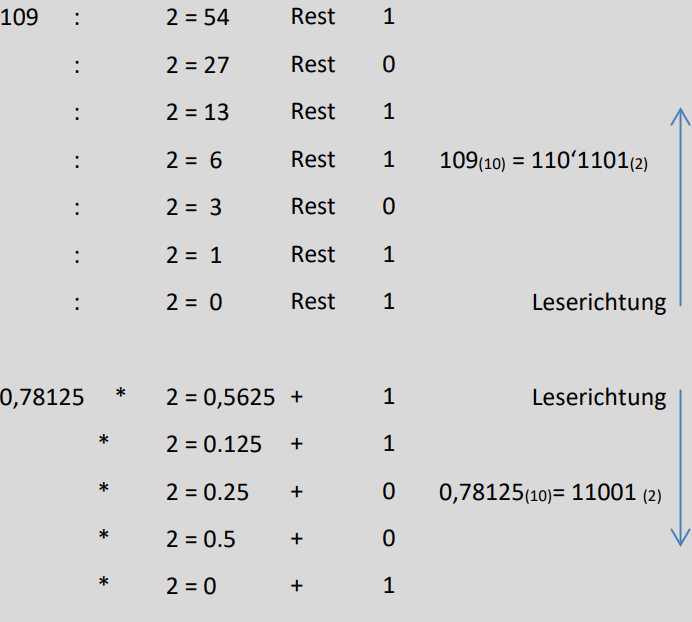
\includegraphics[width=0.25\textwidth]{Umwandlung.PNG}
\columnbreak
\subsection{Einerkomplement}
Alle Bits werden invertiert wenn ein Bit negativ gemacht wird.
\begin{itemize}
    \item Vorteil: Vorzeichen am ersten Bit erkennbar
    \item Nachteil: 0 existiert 2 mal
\end{itemize}
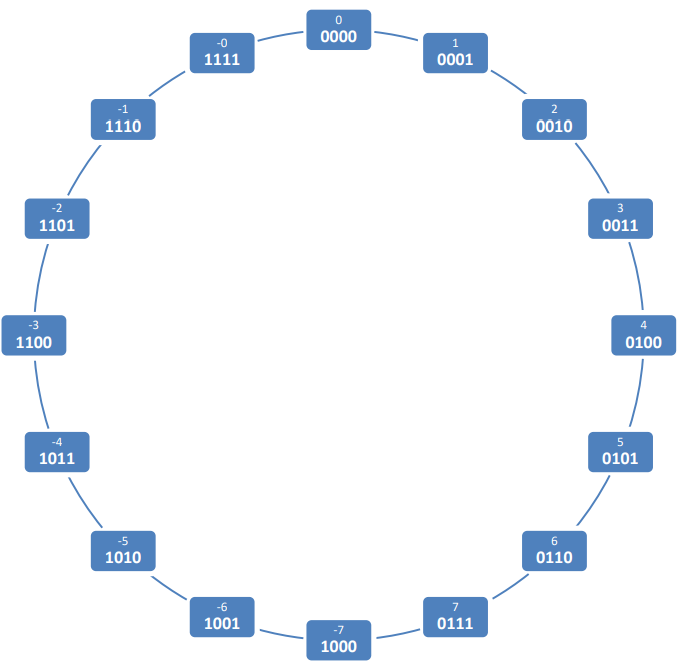
\includegraphics[width=0.25\textwidth]{Einerkomplement.PNG}
\columnbreak
\subsection{Zweierkomplement}
Das Zweierkomplement wird durch Invertieren aller Bits der
positiven Zahl und der Addition von 1 gebildet.
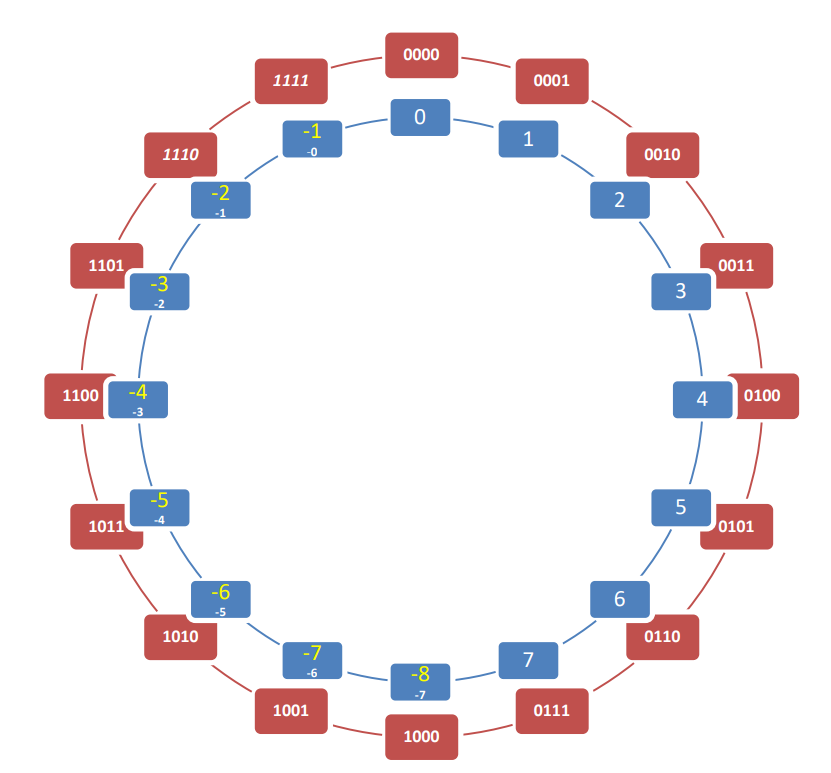
\includegraphics[width=0.3\textwidth]{Zweirkomplement.PNG}
\end{multicols}
\begin{center}
    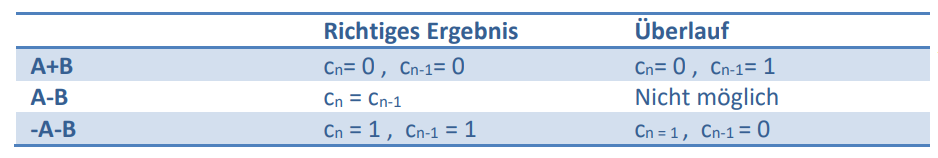
\includegraphics[width=0.6\textwidth]{Bereichsuberschreitung.PNG}
\end{center}
\section{Schaltalgebra}
\subsection{Rechenregeln}
    \textbf{Vereinfachungen}
    \begin{center}
         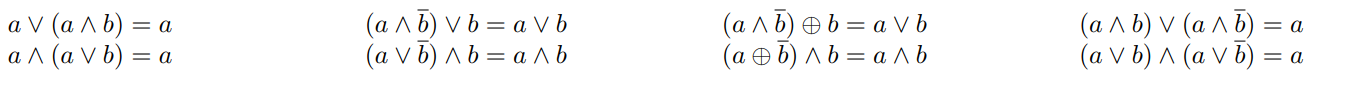
\includegraphics[width=\textwidth]{Vereinfachung.PNG}
    \end{center}
    \subsection{Shannon / De Morgan}
    Shannon: Alle Eingänge und Ausgänge invertieren und "und" mit "oder" tauschen \\
    DeMorgan: Alles invertieren und "und" mit "oder" tauschen
    \begin{center}
        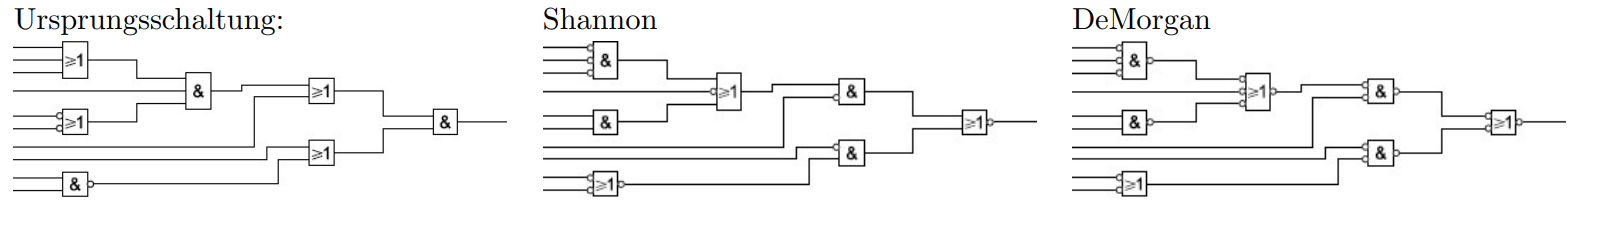
\includegraphics[width=\textwidth]{Shannon_DeMorgan.PNG}
    \end{center}
\begin{multicols}{2}
\subsection{KDNF}
Bei allen Spalten der Wahrheitstabelle bei welcher eine 1 oder "dont care" ausgeben wird, wird mit einem "UND" die Variabeln zusammengenommen danach werden alle Spalten mit einem "ODER" verknüpft.
\columnbreak
\subsection{KKNF}
Bei allen Spalten der Wahrheitstablle bei welcher eine 0 oder "dont care" ausgeben wird, wird mit einem "ODER" die \textbf{INVERTIERTEN} Variabeln zusammengenommen danach werden alle Spalten mit einem "UND" verknüpft.
\end{multicols}
Dont cares werden mit einer eckigen Klammer [ ] gekennzeichnet
\begin{multicols}{2}
    \subsection{KV- Diagramm}
\begin{itemize}
    \item Wahrheitstabelle aufstellen
    \item KV Diagramm entsprechend Nummern einfüllen
    \item Möglichst grosse 2*n Gruppen von 0ern beim KKNF oder von 1ern beim KDNF (Dont cares dürfen beinhaltet sein)
\end{itemize}

\columnbreak
\begin{center}
    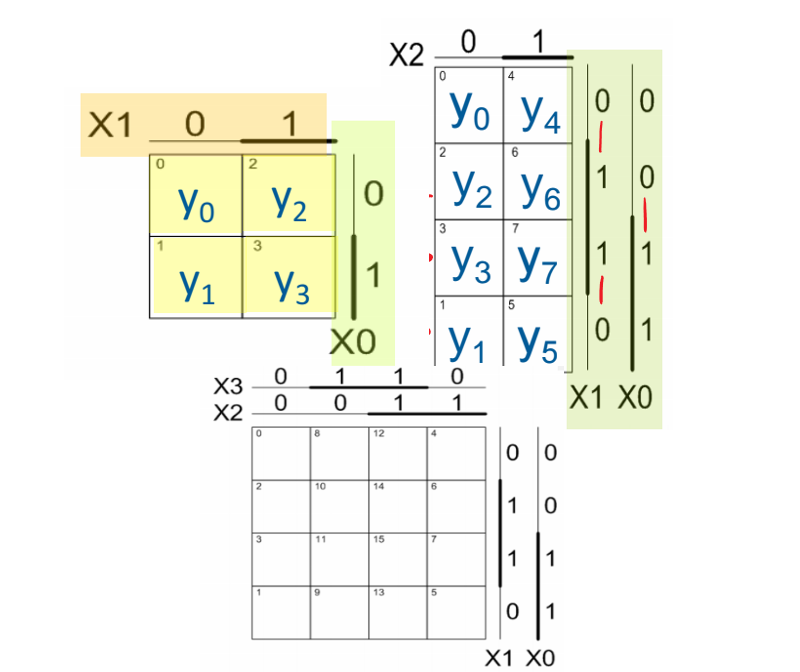
\includegraphics[width=0.25\textwidth]{KV006.png}
\end{center}
\end{multicols}
\subsection{Schaltsymbole}
\begin{multicols}{2}
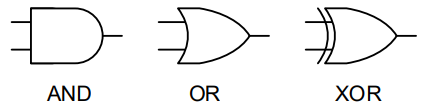
\includegraphics[width=0.25\textwidth]{Zeichen.PNG}
\columnbreak
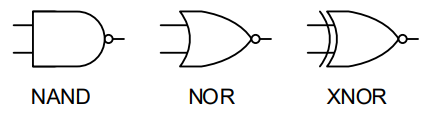
\includegraphics[width=0.25\textwidth]{Zeichen2.PNG}
\end{multicols}
\section{Schaltungstechnologie}
\subsection{CMOS - Logik}
\begin{multicols}{2}
    Zwei verschiedene Arten: p- Kanal und n- Kanal Transistoren.\textbf{n - Kanal} Transistor leited bei \textbf{positver Gate Source Spannung} und umgekehrt.
    \columnbreak
    \begin{center}
    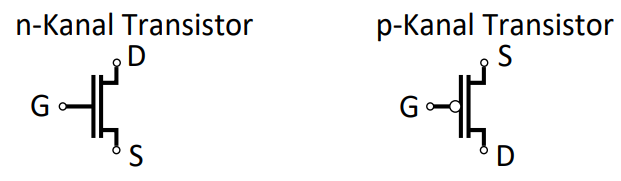
\includegraphics[width=0.3\textwidth]{np_Trans.PNG}
\end{center}    
\end{multicols}
CMOS Logikschaltungen bestehen immer aus einem PMOS (oben VCC) und einem dualen NMOS (GND) Teil. Kein statischen Stromverbrauch \\
\textbf{Komplexität: } 4 Transistoren sind ein Gatterequivalent (GE) 
\begin{multicols}{4}
[\subsection{CMOS Realisierung logischer Funktionen}
Es dürfen nie die Ausgänge von Transistoren direkt zusammengeschaltet werden.
]
\subsection{Inverter}
GE = 0.5
\begin{center}
    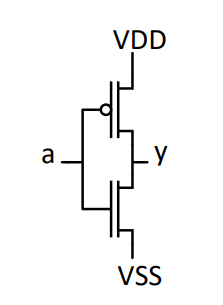
\includegraphics[width=0.1\textwidth]{Inverter.PNG}
\end{center}
\columnbreak
\subsection{NAND}
GE = 1
\begin{center}
    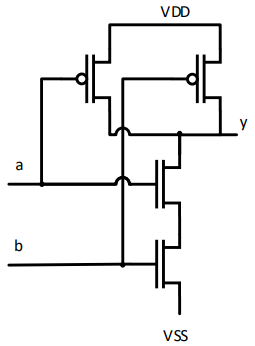
\includegraphics[width=0.1\textwidth]{NAND.PNG}
\end{center}
\columnbreak
\subsection{NOR}
GE = 1
\begin{center}
    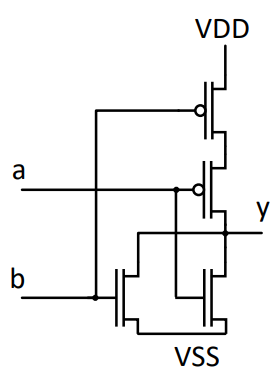
\includegraphics[width=0.1\textwidth]{NOR.PNG}
\end{center}
\columnbreak
\subsection{XOR}
GE = 2
\begin{center}
    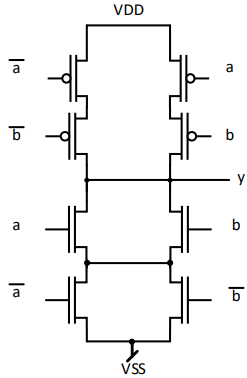
\includegraphics[width=0.1\textwidth]{XOR_Trans.PNG}
\end{center}
\end{multicols}
\begin{multicols}{2}
\subsection{Übergangszeit}
Ein Wechsel von einem Wert auf ein neuen benötigt etwas Zeit, diese Zeit wird Überganszeit (Transition Time) genannt.
\begin{center}
    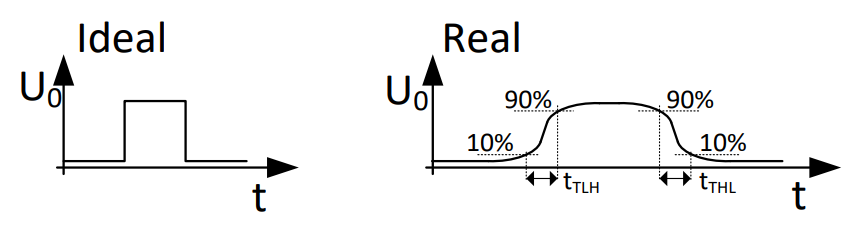
\includegraphics[width=0.3 \textwidth]{TransitionTime.PNG}
\end{center}
\columnbreak
\subsection{Verzögerungszeit}
Die Verzögerungszeit (Propagation Delay) bezeichnet die Differenz des Eingangssignal zum Ausgangssignal.
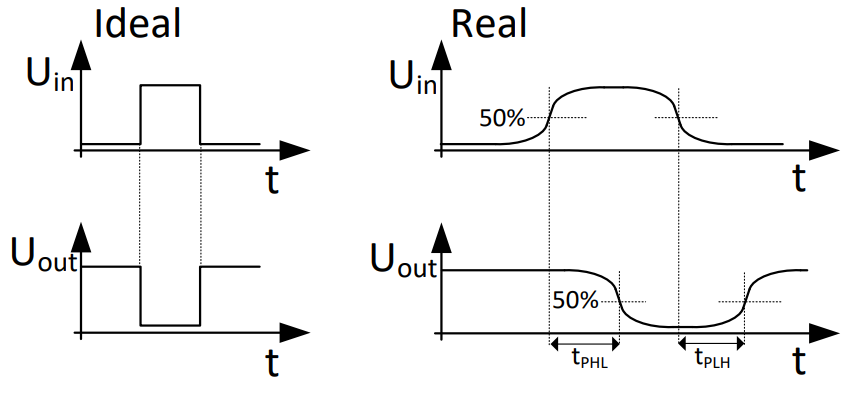
\includegraphics[width=0.3\textwidth]{PropagationDelay.PNG}
\end{multicols}
\subsection{Hazards}
In digitalen Systemen kann es durch unterschiedliche Laufzeitpfade zu
kritischen Wettrennen von Signalen kommen. Solche Laufzeiteffekte führen zu unerwünschten Signalzwischenwerten, sogenannten Hazards.
\begin{multicols}{2}
\subsection{Statische Hazards}
Ein Funktionswert \textbf{ändert einmal kurzzeitig seinen Pegel} wenn eine Eingangsvariable den Pegel ändert, obwohl \textbf{dies nicht sein sollte}. 
\columnbreak
\subsection{Dynamische Hazards}
Ein Funktionswert ändert \textbf{mehrmalskurzzeitig seinen Pegel} nachdem sich eine Eingangsvariablen geändert hat, obwohl der Ausgang sich \textbf{nur einmal} hätte ändern müssen.
\end{multicols}
\section{Grundlagen sequenzieller Systeme}
Sequenzielle Systeme haben eine Clock oder ein Taktsignal. Das Taktsignal ist ein binäre Signal, das in regelmässiger Abfolge zwischen zwei Zuständen hin und her pendelt. $f = \frac{1}{T}$
\subsection{Unterschied Flip - Flop / Latch}
\textbf{Taktflankengesteuerte} Speicherelemente werden \textbf{Flip-Flops} genannt. \\
\textbf{Taktzustandsgesteuerte} Speicherelemente werden \textbf{Latches} genannt
\begin{multicols}{2}
[
\subsection{Latches / Flip Flops}
]
\subsubsection{RS-Latch}
Der Zustand S = 1 und R = 1 ist undefiniert.
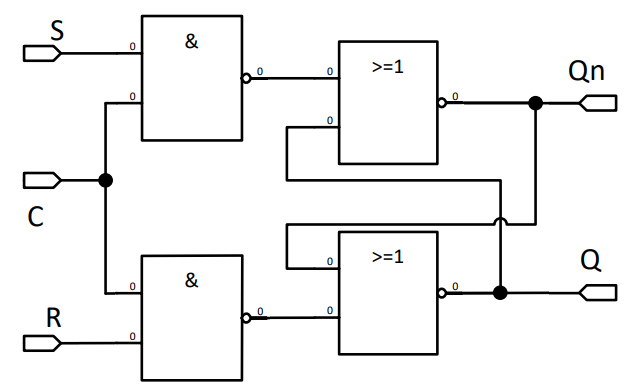
\includegraphics[width=0.2\textwidth]{RS-Latch.PNG}
\columnbreak
\subsubsection{D-Latch}
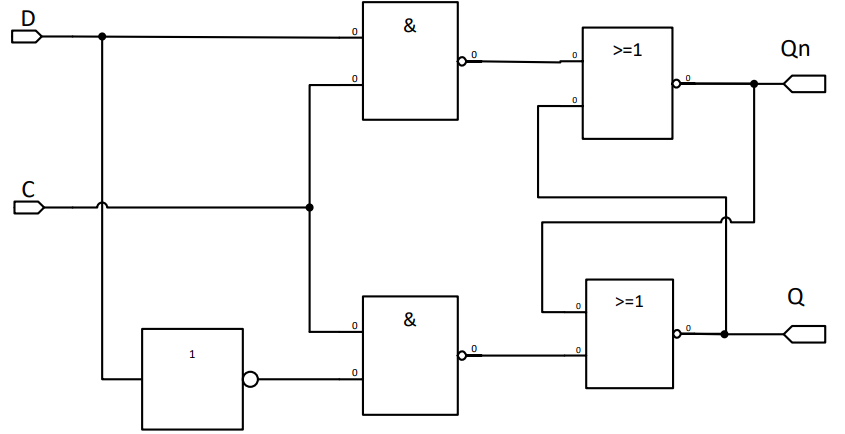
\includegraphics[width=0.2\textwidth]{D-Latch.PNG}
\end{multicols}
\subsection{D-Flip Flop}
\begin{center}
    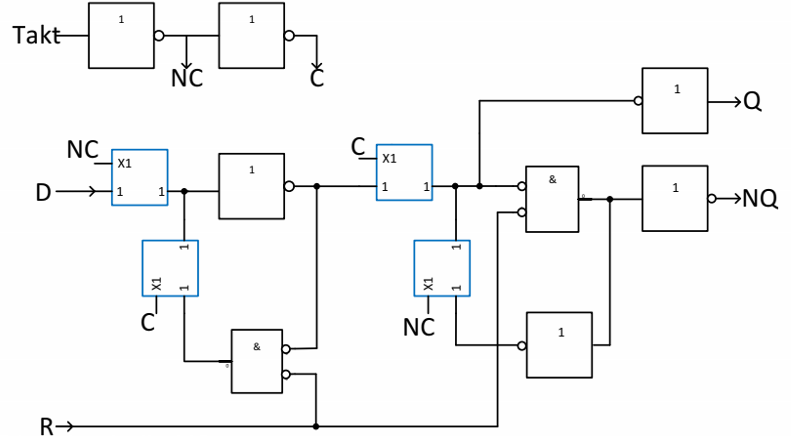
\includegraphics[width=0.3\textwidth]{DFlipFlop.PNG}
\end{center}
\newpage
\begin{multicols}{2}
    \begin{equation}
    q = \frac{2^k!}{(2^k - p)!}
    \end{equation}
    \begin{center}
    k = Benötigte Speicherstellen = $log_2(s)$ \\
p = Anzahl Zustände
\end{center}
\columnbreak
\subsubsection{Setup- und Hold-Zeit}
Die \textbf{Setup-Zeit} ist die Zeit in welcher das Eingangssignal vor der aktiven Taktflanke einer Schaltung stabil sein muss. \\
Bei der \textbf{Hold-Zeit} ist dies nach der aktiven Taktflanke.
\begin{center}
    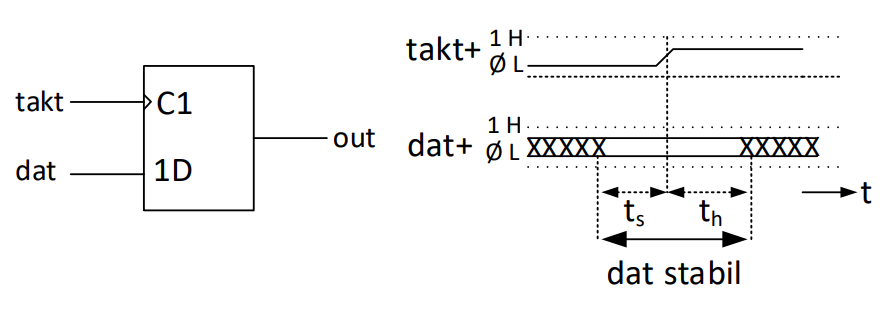
\includegraphics[width=0.2\textwidth]{Setup-HoldTime.PNG}
\end{center}
\end{multicols}
RAM $\rightarrow$ Read only ROM $\rightarrow$ Read and Write DRAM $\rightarrow$ Zustand geht verloren SRAM $\rightarrow$ Bleibt solange Stromversorgung da
\begin{multicols}{2}
\subsubsection{Zustandstabelle}
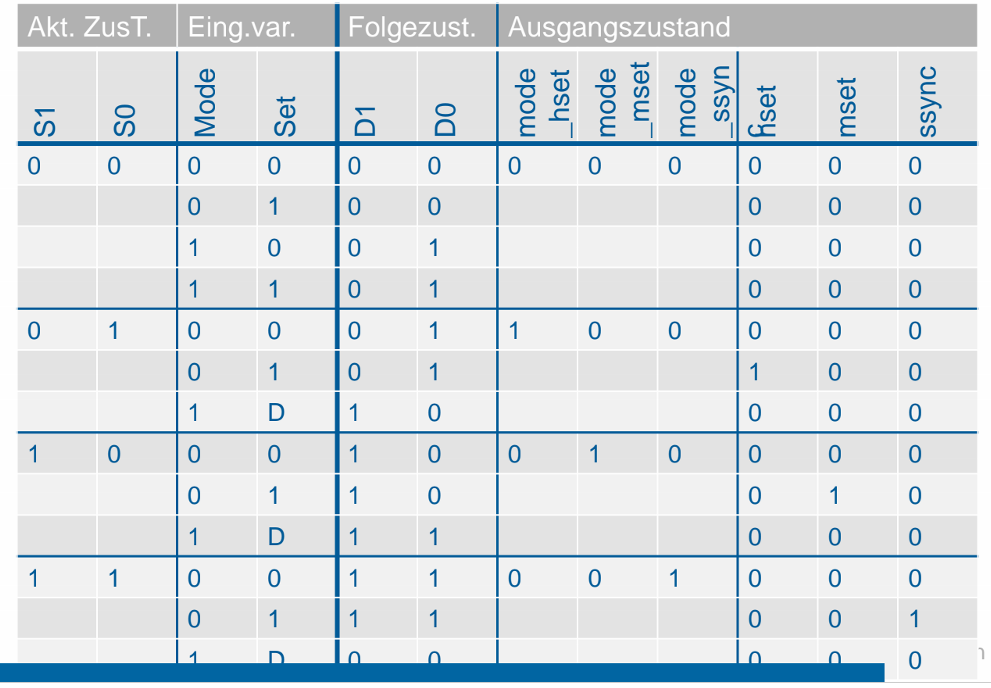
\includegraphics[width=0.3\textwidth]{Zustandstabelle.PNG}
\columnbreak
\subsection{Zustandsdiagramm}
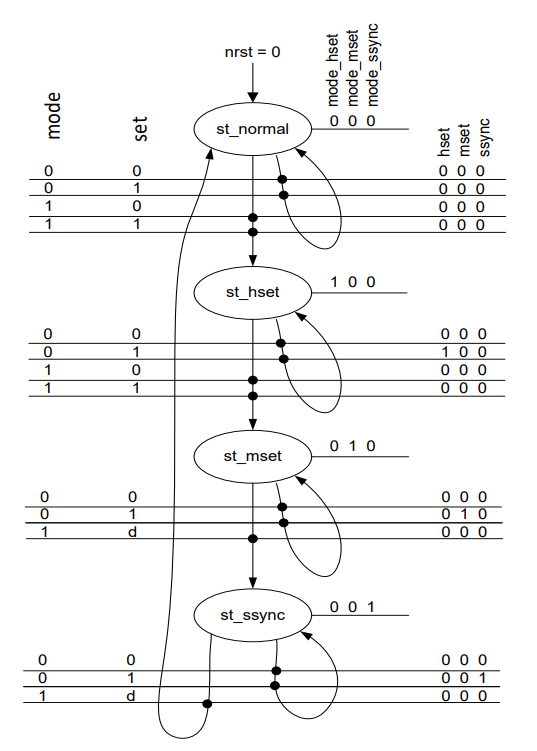
\includegraphics[width=0.2\textwidth,angle=90]{Zustandsdiagramm.PNG}
\end{multicols}
\begin{multicols}{3}
    x $\rightarrow$ Eingangsvektor \\
    m $\rightarrow$ Anzahl Eingänge\\
    y $\rightarrow$ Ausgangsvektor \\
    n $\rightarrow$ Anzahl Ausgänge \\
    s $\rightarrow$ Zustandsvektor\\
    d $\rightarrow$ Folgezustand\\
    F $\rightarrow$ Funktion Ausgänge \\
    G $\rightarrow$ Speicheransteuerung \\
    Z $\rightarrow$ Zustandsspeicher
\end{multicols}
\begin{multicols}{3}
\subsubsection{Mealy-System}
Abhängig von: Zustand / Eingang
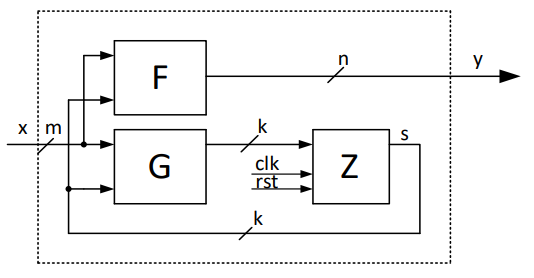
\includegraphics[width=0.2\textwidth]{Mealy.PNG}
\columnbreak
\subsubsection{Moore - System}
Abhängig von: Zustand
\begin{center}
    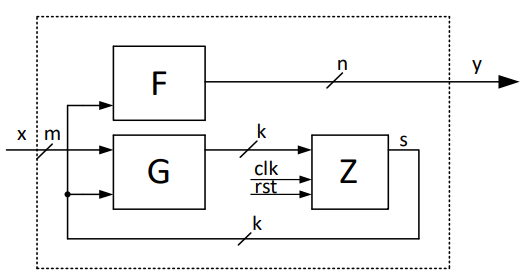
\includegraphics[width=0.2\textwidth]{Moore.PNG}
\end{center}
\subsection{Medwedjew - System}
Die primären Ausgänge entsprechen
dem Zustandsvektor s
\begin{center}
    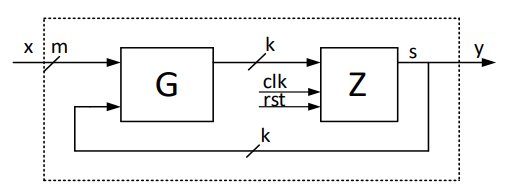
\includegraphics[width=0.2\textwidth]{Medjedew.PNG}
\end{center}
\end{multicols}
\begin{multicols}{2}
    \begin{center}
        \textbf{Zeit Mealy} \\
    Berechnung max. Clockfreqeunz kompliziert. Meherere Mealy-Maschinen können sehr langen Signalpfad erzeugen
    \end{center}
    \columnbreak
    \begin{center}
            \textbf{Zeit Moore / Medwedjew} \\
    Mehrere Moore-Maschinen erzeugen Verzögerung im Sinne von mehreren Takten.
    \end{center}
\end{multicols}
\begin{multicols}{3}
    [\subsection{Zustandscodierung}]
    \subsubsection{Binär}
    Das Standard binär System wird für die Codierung verwendet
    \columnbreak
    \subsubsection{ONE - HOT}
    Nur ein Bit ist eine 1
    \subsubsection{ONE - COLD}
    Nur ein Bit ist eine 0
\end{multicols}
\end{document}
